\documentclass[kulak]{kulakarticle} % options: kulak (default) or kul

\usepackage[dutch]{babel}
\usepackage{amssymb, amsthm, amsmath}
\usepackage{siunitx}
\usepackage{graphicx}

\title{Examen Conceptuele Natuurkunde}
\author{Vincent Van Schependom}
\date{12 januari 2024}
\address{\textbf{Conceptuele Natuurkunde} \\\textbf{met technische toepassingen}\\
	Prof. David Dudal}

\begin{document}

\maketitle

\section{Theorie (10pt)}

\subsection{Vraag 1: de centrale elastische botsing (3pt)}

Toon aan dat de kinetische energie-overdracht van massa \(m_1\) naar massa \(m_2\) bij een centrale elastische botsing wordt gegeven door \[\frac{2m_1m_2}{(m_1+m_2)^2}(v_{1i}-v_{2i})(m_1v_{1i}+m_2v_{2i})\] indien zowel de kinetische energie als de impuls van het systeem behouden blijft.

\subsection{Vraag 2: slingers (3pt)}

De fysische slinger is een vormvast voorwerp dat vrij kan roteren rond een vaste horizontale rotatie-as \(R\) onder invloed van de zwaartekracht \(\vec{G}\). Stel de bewegingsvergelijking op van de slinger, met lengte \(l\), massa \(m\) en traagheidsmoment \(I\).\\

\noindent Hoe verschilt deze bewegingsvergelijking van die van de wiskundige/ideale slinger? Geef ook hiervan de bewegingsvergelijking en vergelijk met die van de fysische slinger.\\

\noindent Ga er bij beide slingers vanuit dat de beginuitwijking zeer klein is.

\subsection{Vraag 3: elektromagnetisme (4pt)}

\begin{enumerate}
	\item Wat gebeurt er als er zich een puntlading binnenin een geleider in rust bevindt? \\\textit{Dit stond er niet bij, maar deze vraag komt neer op: verklaar waarom excess-lading zich slechts aan de rand van een geleider in rust kan bevinden.}
	\item Hoe staat het elektrisch veld op de rand van zo'n geleider? Verklaar en bewijs waarom dit zo is.
	\item Wat kan er gebeuren indien het elektrisch veld te sterk wordt?
	\item Stel dat er zich een positieve lading \(q^+\) in de holte van een sferische geleider in rust bevindt. Hoe zal de elektrische veldconfiguratie er dan uitzien?
\end{enumerate}

\newpage

\section{Oefeningen (6pt)}

\subsection{Vraag 1: mechanica}

Een kar met een kanon erop schiet een projectiel, zijnde een kanonskogel, af. Het systeem van de kar en het kanon kan horizontaal vrij bewegen en is aan de voorkant bevestigt aan een veer, die initieel in rust is.\\

\noindent Gegeven:

\begin{itemize}
	\item Massa van de kar met het kanon: \(m_k=5000\)\si{kg}
	\item Massa van de kogel: \(m_p = 200\)\si{kg}
	\item Snelheid van de kogel: \(v_p= 125\)\si{m/s}
	\item Starthoogte van de kogel: \(1\)\si{m}
	\item Veerconstante: \(k=4.00\cdot10^4\)\si{N/m}
	\item Hoek van het kanon met de kar: \(\theta=45\)°
\end{itemize}

\noindent Gevraagd:

\begin{enumerate}
	\item Hoe ver zal de kogel neerkomen?
	\item Hoe groot is de terugslagsnelheid \(v_k\) van het karretje en het kanon na het afvuren van de kogel?
	\item Hoe ver zal de veer maximaal uitgerokken worden?
	\item Wat is de maximale kracht die de veer op de kar uitoefent?
\end{enumerate}

\subsection{Vraag 2: elektromagnetisme}

In een netwerk hebben alle weerstanden weerstand \(R\), buiten eentje, die heeft weerstand \(R'\). We leggen een spanningsbron aan met EMS \(\varepsilon\). Aan de hand hiervan bepalen we de stromen doorheen de verschillende takken. Leid hieruit dan de subsitutieweerstand \(R_{\text{eq}}\) af.

\begin{figure}[h!]
	\centering
	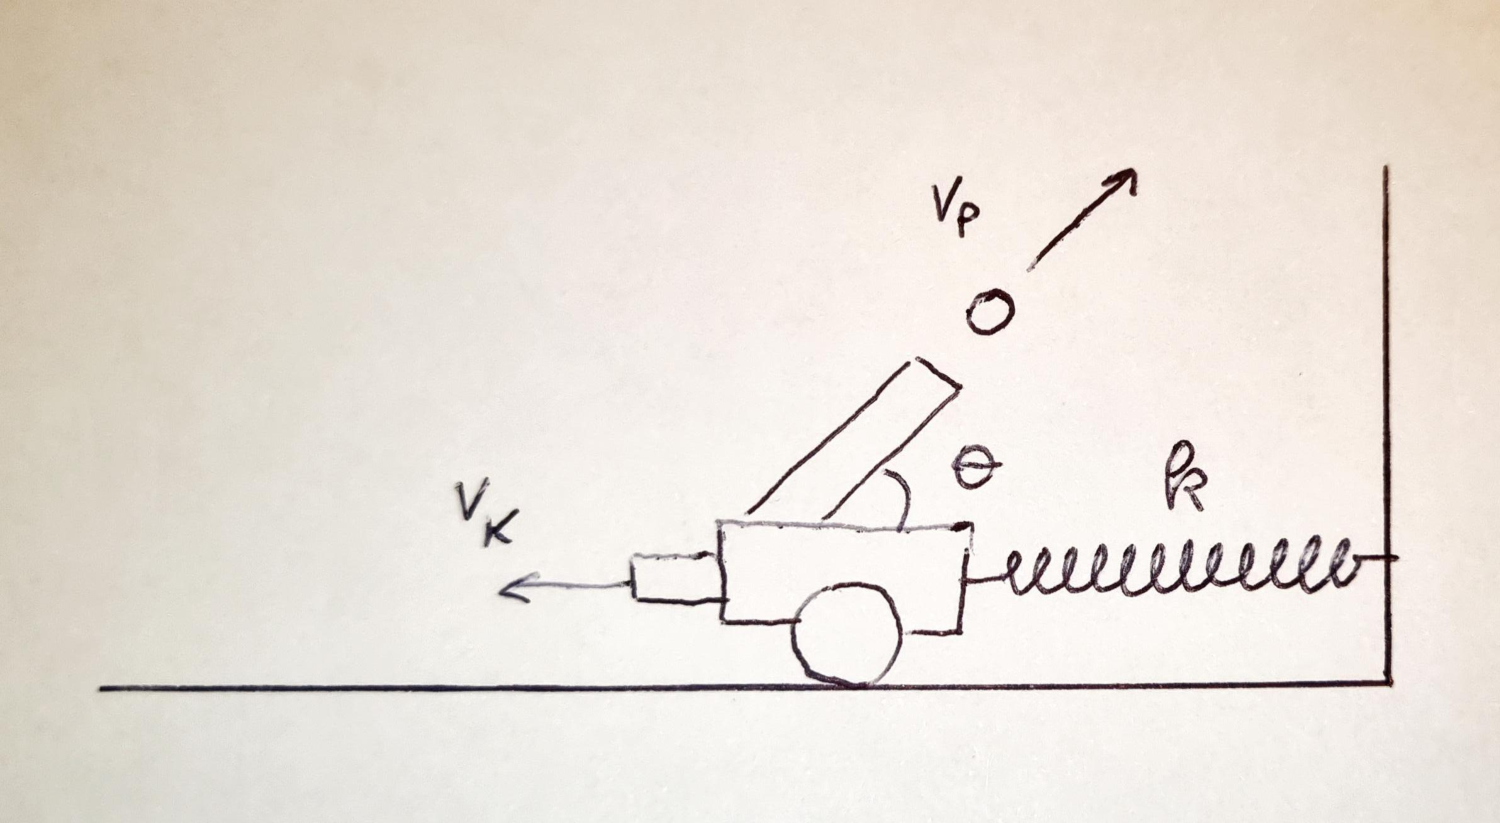
\includegraphics[height=.3\textwidth]{oef1}\hspace{1cm}
	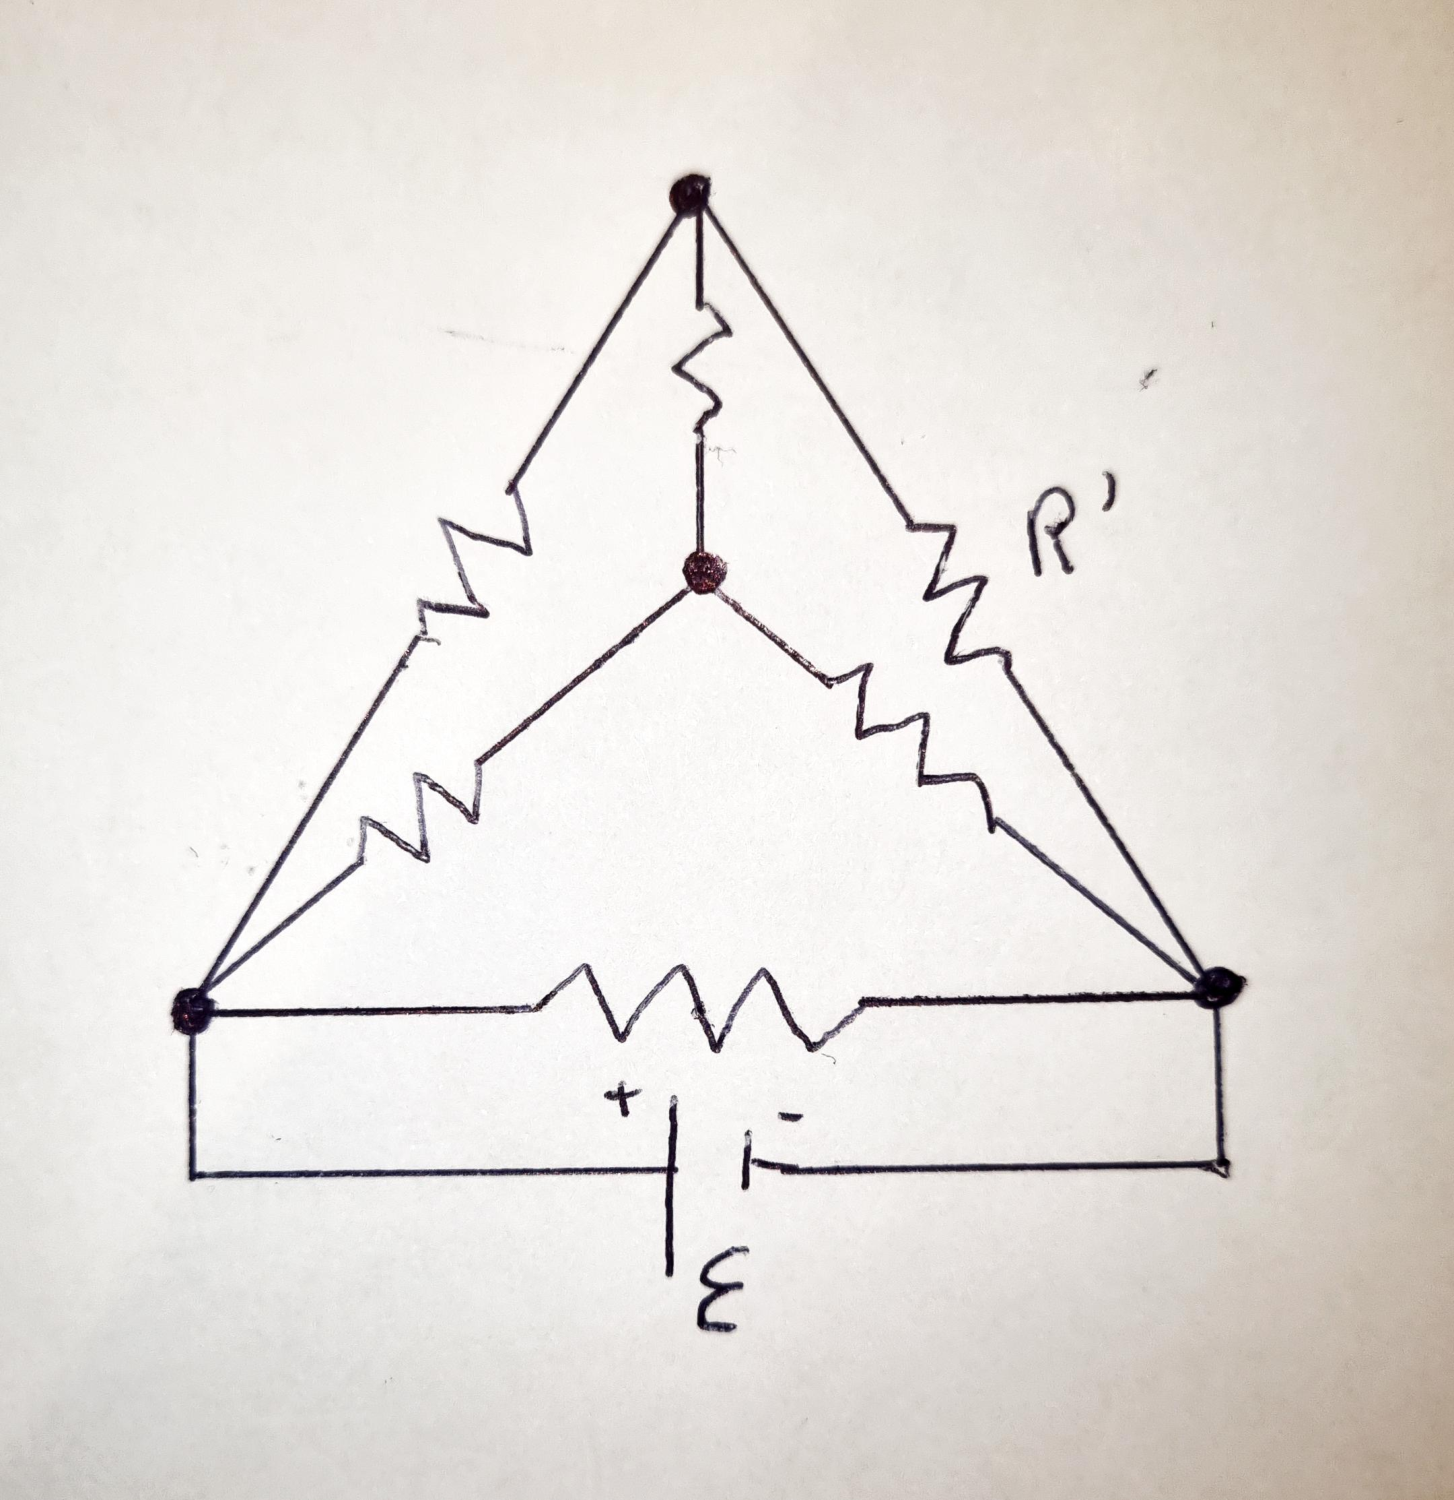
\includegraphics[height=.3\textwidth]{oef2}
\end{figure}

\section{Practica (4pt)}

De practica over het Dopplereffect en de Wet van Faraday stonden op 4 punten.

\end{document}
